\documentclass[ukenglish]{beamer}

%%% Dichiarazione dei pacchetti standard.
\usepackage[utf8x]{inputenc}
\usepackage{graphicx}    % inclusione graph images (eps)
\usepackage{units}
\usepackage{url}
\setbeamertemplate{navigation symbols}{\insertframenumber} 

\usetheme{Frankfurt}
\usecolortheme{wolverine}
    
%%% Titolo e autore.
\title{Prospects in the search for top partners}
\author{Matteo Abis\\
\url{matteo.abis@cern.ch}}
\institute{Università di Padova}
\date{\today}

\begin{document}
\begin{frame}
  \titlepage
\end{frame}
 
\begin{frame}
    \frametitle{Goal statement.}
    Conclusion and refinement of the analysis of top partner events.
    $T \bar T \longrightarrow \ell \ell + n$ jets.
    \begin{itemize}
        \item validate the MC samples;
        \item import the existing analysis into the CMGTools framework;
        \item refine the analysis with razor-like variables.
    \end{itemize}
\end{frame}

\begin{frame}
    \frametitle{Validation of the MC samples.}
\begin{itemize}
    \item bugs in the older samples;
    \item independent crosscheck of LHE files;
    \item thank you Aram for the new samples and validation;
    \item fast or full simulation at some point.
\end{itemize}
\end{frame}

\begin{frame}
    \frametitle{Validation of the MC samples.}
    \framesubtitle{This is happening as we speak.}
    from file:
    \url{/castor/cern.ch/user/a/avetisya/TopPartners}\\
    \url{/NewSampleTest/PostProc_T53_PairProd_400.lhe.gz}
    \begin{figure}[h]
        \begin{center}
            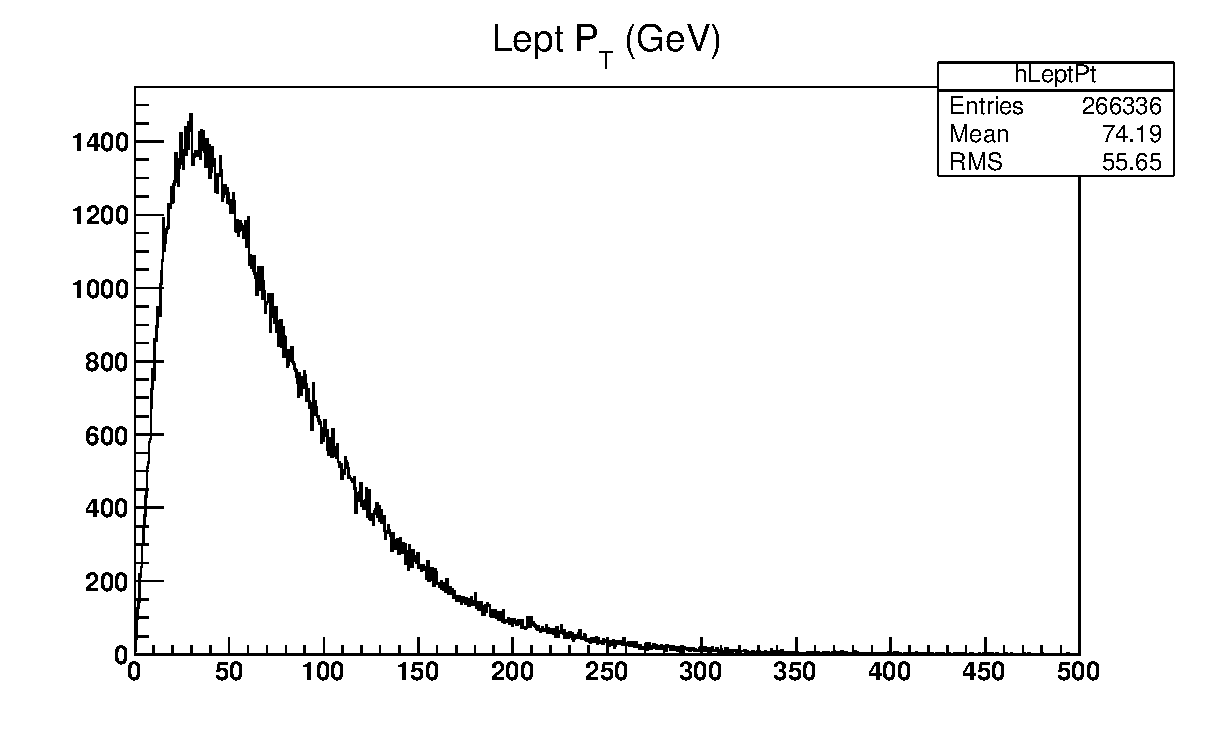
\includegraphics[width=.3\textwidth]{lepton_pt.eps}
            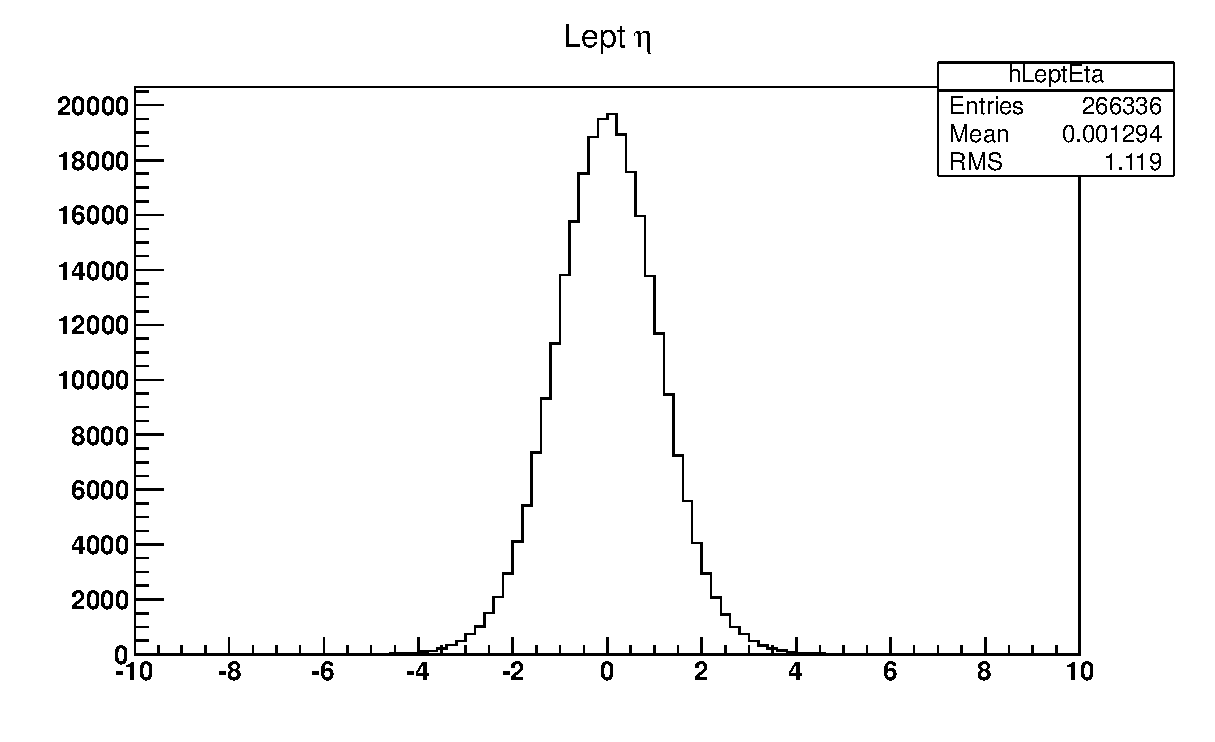
\includegraphics[width=.3\textwidth]{lepton_eta.eps}
            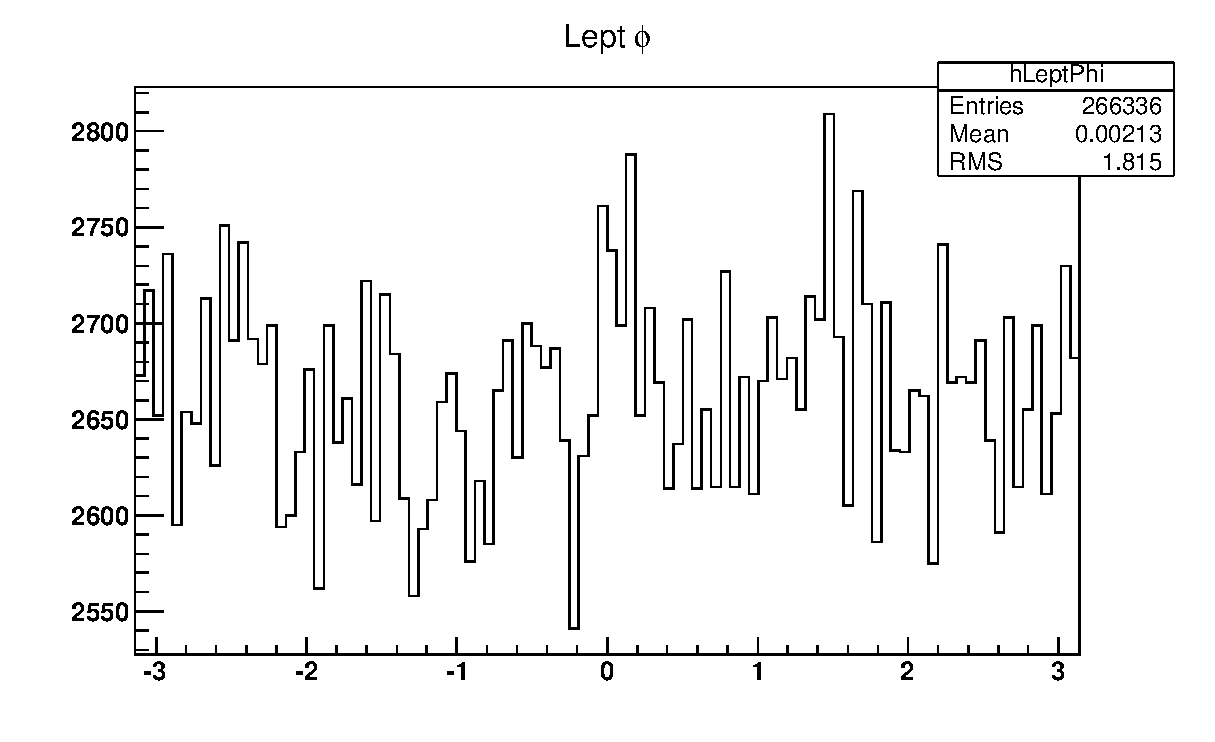
\includegraphics[width=.3\textwidth]{lepton_phi.eps}
        \end{center}
    \end{figure}
\end{frame}

\begin{frame}
    \frametitle{Importing the analysis into the CMGTools framework.}
    \begin{itemize}
        \item work done by Massimo Nespolo with his own framework;
        \item reconsider and refine cuts, particle identification.
            \begin{itemize}
                \item using standard collections \texttt{cmg::Electrons},
                    \texttt{Muons}\dots;
                \item MET?
                \item $b$ tagging?
            \end{itemize}
    \end{itemize}
\end{frame}

\begin{frame}
    \frametitle{Future enhancements: razor variables.}
    \begin{itemize}
        \item already employed in the search for supersymmetric particles;
        \item \alert{asymmetric nature of the event!}
    \end{itemize}
\end{frame}
\end{document}
